\chapter{Ex-Vivo Renal MRI}
\label{chap:ex}
\newpage
\begin{abstract}
	Despite recent developments in quantitative renal \ac{MRI} the current clinical standard for diagnosis of renal pathologies is limited to collection of a  biopsy for histology, an invasive procedure that is not without risks and highly susceptible to sampling bias. To aid the clinical adoption of renal \ac{MRI} the association between \ac{MRI} contrasts and underlying histology must be better understood.	
	
	By scanning subjects who are due to undergo a nephrectomy as part of their standard clinical care, the same kidney can be imaged in-vivo using state of the art protocols prior to organ removal. Once the kidney has been removed, the explant can be imaged ex-vivo in exquisite detail to collect the highest quality of \ac{MRI} data, this can then be correlated to  histological analysis. These three complimentary streams of data will lead to a better understanding of the \ac{MRI} parameters and validate quantitative \ac{MRI} in the clinic. In future, such and ex-vivo \ac{MRI} protocol could also be used to assess the viability of kidney grafts prior to transplant. Here a matched ex-vivo and in-vivo multiparametric renal \ac{MRI} protocol and advance analysis methods are developed for future clinical studies.
	
	\textit{This work was presented at the \ac{ISMRM} 27th Annual Meeting, 2019 \cite{daniel_effects_2019} and \ac{UKKW} 2019 \cite{kazmi_determining_2019-1}. The bespoke analysis pipelines and software developed here have been incorporated into the development of The \ac{UKAT} \cite{nery_ukrin_2020}. This work will be presented at the \ac{ISMRM} 29th Annual Meeting, 2021, \cite{daniel_ukrin_2021}.}
\end{abstract}
\acresetall
\newpage
\section{Introduction}

A recurring theme in renal \ac{MRI} studies is the limitations imposed by respiratory motion. Sequences must either be optimised and accelerated to fit within a breath-hold, hugely slowed down through the use of respiratory triggering or accepting that motion artefacts are inevitable during a free-breathing acquisition. Additionally the common trade-off in \ac{MRI} between voxel size, \ac{FOV} and acquisition time becomes all the more limiting. While these issues are ever-present in day-to-day clinical practice, to validate methods for clinical adoption it is desirable to acquire data of higher quality (spatial resolution and multiple contrasts) in the research phase. This can provide a detailed understanding of the spatial variance of \ac{MRI} contrasts across the whole kidney to inform lower resolution clinical scans.

In this chapter, techniques for ex-vivo renal \ac{MRI} are developed. These allow research to be conducted without the limitations imposed by respiratory motion to study the kidney in great detail, develop new imaging protocols and understand multiparametric \ac{MRI} contrast and its association with underlying histological features. In the future, this ex-vivo imaging protocol, could be used to compare in-vivo and ex-vivo measures in patients undergoing a nephrectomy or used in transplant centres to assess allograft viability prior to transplant.

\subsection{Validation of Multiparametric MRI via a Nephrectomy Model}

Blood and urine tests are commonly used to assess renal health and function however, these are indirect measures and given no indication as to the health of individual kidneys. Consequently, the gold standard in renal diagnostics is a biopsy followed by histological analysis. During a renal biopsy, an area on the patients back is injected with local anaesthetic then, using ultrasound as a guide, a biopsy needle is inserted into the kidney to remove a sample of the tissue. Acquiring the biopsy takes approximately half an hour. After the sample is removed the patient is then asked to lie in bed for several hours to minimise the risk of internal bleeding. In approximately 1~\% of patients, the bleeding caused will require a blood transfusion and approximately 0.5~\% of patients will require embolisation. While these risks are relatively small, the procedure is still an invasive, destructive and time consuming one for the patient thus making it poorly suited for longitudinal monitoring of renal health. Additionally, this method of biopsy is not viable for some patients such as those with coagulopathy or thrombocytopenia due to the increased risk if a hemorrhage occurs, or those that are unable to lie prone such as those patients who are intubated for respiratory assistance \cite{rathod_safety_2017}. While techniques such as the transjugular renal biopsy have been developed (albeit accidentally after taking a wrong turn at the portal vein while trying to acquire a liver biopsy \cite{mal_transjugular_1990}) to serve these patients, this is a more technically complicated procedure. Finally, the samples acquired via biopsy are very small and thus are often not representative of the entirety of the kidney biopsied, let alone both kidneys.

These drawbacks of biopsy have provided a key incentive for the development of multiparametric renal \ac{MRI} protocols which could prove to be advantageous for both clinical decision making and patient care and well-being. A key aspect in the widespread adoption of \ac{MRI} into renal clinical practice, is a full understanding of the interplay between the current histological measures and \ac{MRI} contrasts. While it is possible to correlate biopsy results with \ac{MRI} findings and gain some information as to how different \ac{MRI} measurements vary with tissue properties, this suffers from the small tissue sampling volumes outlined above \cite{leung_could_2017}. An alternative paradigm is the nephrectomy model where it may be possible to scan the kidney in-vivo to collect multiparametric renal \ac{MRI} data, and then scan the organ ex-vivo to acquire exquisite \ac{MRI} data of a far higher spatial resolution or with many more contrasts than would be possible in-vivo and then perform whole organ histology on the tissue, Figure \ref{fig:ex_neph_flowchart}. These three streams of complimentary data, all acquired from the same organ, allow direct relationships to be formed while relating the data back to clinically feasible, lower spatial resolution measures.

\begin{figure}[H]
	\centering
	\includegraphics[width=1\textwidth]{Neph/Neph_Flowchart.eps}
	\caption{Flowchart showing an overview of the nephrectomy paradigm.}
	\label{fig:ex_neph_flowchart}	
\end{figure}


One of the first studies correlating in-vivo multiparametric \ac{MRI} with renal histology was by Inoue \textit{et al}, who found a statistically significant negative correlation between fibrosis area, as determined from a renal biopsy stained with Masson's trichrome, and \ac{ADC} and \ttwostar in 37 \ac{CKD} patients \cite{inoue_noninvasive_2011}. This was confirmed by Zhao \textit{et al}, who also reported a strong negative correlation between \ac{ADC} of both the renal cortex and medulla and histopathological fibrosis score in 25 \ac{CKD} patients \cite{zhao_assessment_2014}; this study used a more comprehensive histopathology protocol. Feng \textit{et al} also showed a negative correlation between glomerulosclerosis, fibrosis, \ac{FA} and \ac{ADC} in \ac{CKD} subjects \cite{feng_dti_2015}. Friedli \textit{et al} published a significant positive correlation between cortical-medullary differences in \tone and fibrosis and negative correlation between cortical-medullary differences in  \ac{ADC} and fibrosis, this was first published in rats, where \ac{MRI} data was correlated with histology of whole organs rather than just biopsy samples \cite{friedli_new_2016}. The same group then validated this finding in 164 human subjects, correlating \ac{MRI} measures with biopsy rather than whole organ measures \cite{berchtold_validation_2020}.

Outside of the renal \ac{MRI} community, studies have been done with registered whole-mount histology and both in-vivo and ex-vivo \ac{MRI}. Jafari \textit{et al} performed volume matched ex-vivo \ac{QSM} and \ttwostar mapping with whole explant histopathology of the liver using the histopathology results to validate predictions of fibrosis using \ac{MRI} \cite{jafari_integrated_2021}. The University of British Columbia group have carried out extensive work correlating histopathology of whole prostatectomy samples with in-vivo \ac{MRI} \cite{sabouri_mr_2017, dhatt_mri_2020}. The same group have also made use of ex-vivo scanning techniques to correlate histopathology with 7T narrow-bore ex-vivo data and 3T in-vivo data \cite{uribe_vivo_2015}. The use of matched histology and \ac{MRI} data is now becoming well established in the neuroimaging field \cite{lazari_can_2021} with studies correlating histopathology with diffusion measures \cite{peters_white_2019, moll_multiple_2011, howard_joint_2019, mollink_white_2019}, magnetisation transfer \cite{mottershead_high_2003, seewann_diffusely_2009}, \ac{QSM} \cite{hametner_influence_2018, stuber_myelin_2014} and relaxometry measures \cite{bagnato_untangling_2018, reeves_combined_2016}. Additionally, post processing packages have been developed to enable accurate registration of whole mount histopathology and \ac{MRI} data \cite{huszar_tensor_2019, huszar_automated_2019}.

Thus far, no work has been published comparing in-vivo and ex-vivo \ac{MRI} measurements with whole organ renal histology. The ideal paradigm for this work is to scan patients who are undergoing a nephrectomy as part of their standard clinical care, typically for treatment of cancer. Briefly, this method would involve scanning a subject prior to surgery to acquire a multiparametric quantitative \ac{MRI} dataset. The subject will then have part of their kidney removed, the cancerous tissue will be sent for standard lab tests whilst the, non-cancerous tissue will be immersion fixed in formalin. Equivalent scans assessing the same quantitative parameters in-vivo can then be performed ex-vivo at a much higher spatial resolution. Finally, the ex-vivo tissue will be sliced for multi-stain histopathology. This pipeline enables the comparison of tried and tested histological staining with large sample sizes, with in-vivo quantitative \ac{MRI} data; the ex-vivo high spatial resolution data acts as an intermediary which can be directly spatially correlated with histology and in-vivo \ac{MRI} data. To address this goal the development of an ex-vivo \ac{MRI} protocol to image renal tissue is first required.

\newpage
\subsection{Assessment of Allograft Viability}
An alternative use of an ex-vivo \ac{MRI} protocol is the assessment of allograft viability. Availability of transplant kidneys is a major limiting factor in the treatment of many patients with end-stage kidney disease. This results in long times on recipient waiting lists incurring additional risks to the patient from the adverse effects of dialysis upon the body and resulting in higher costs to health services. 

Despite the shortage of donor kidneys, a significant proportion of those kidneys which are donated are currently discarded rather than transplanted. This is due to an understandably cautious approach to acceptance of organs from older donors or those with co-morbidities. However these discarded organs will inevitably span a range of organ qualities, some of which could have been viable grafts. One method of increasing the number of available organs for transplant is to reduce the proportion of discarded kidneys while also avoiding transplanting unviable grafts. To try and assess the viability of marginal organs two methods have been developed using data from the United Kingdom and United States transplant registries. These methods both produce a risk index designed to give 1 for a healthy 40 year old donor, with a risk index < 1 indicating a lower risk donor and a risk index > 1 indicating a higher risk donor. The \ac{UKKDRI} is given by an empirically derived equation based on the risk factors of donor age, history of hypertension, donor weight, days in hospital and the use of adrenaline \cite{watson_simplified_2012} while the \ac{USKDRI} adds an additional ten risk factor to its model \cite{rao_comprehensive_2009}. \ac{ROC} analysis showed an \ac{AUC} of 0.62 and 0.63 for \ac{UKKDRI} and \ac{USKDRI} respectively, indicating both models have limited predictive ability. Model accuracy could likely be highly improved by including measures specific to the kidneys themselves rather than simply demographic and global clinical factors.

\newpage
Between 2009 and 2013, 65~\% of kidney donations came from deceased donors rather than living donors \cite{burton_causes_2019}. As these donations are unplanned, there is a significant time period between kidney retrieval and surgery while a recipient is found, during this time tests could be run on the kidney allograft to assess its viability. One possible modality for such tests is a simple ex-vivo \ac{MRI} of the organ whilst it is on cold storage prior to the transplant.

By developing a quantitative ex-vivo renal \ac{MRI} protocol, the health of the kidney to be transplanted could be assessed while a recipient is being found. \ac{MRI} is ideally suited due to its non-destructive, whole organ coverage, thus avoiding the sampling bias outlined as an issue with biopsy. The results from the \ac{MRI} exam could be used to improve accuracy of the donor risk index and thus result in a lower rate of discarded organs and an increase in long term successful grafts. 

In addition to scanning the allograft ex-vivo, an in-vivo post transplant protocol could be used to assess graft function. By proactively identifying the onset and progression of graft dysfunction, treatment could be modified to extend the life of the transplant. An overview of the potential pipeline is shown in Figure \ref{fig:ex_transplant_flowchart}.
\begin{figure}[H]
	\centering
	\includegraphics[width=0.8\textwidth]{Neph/Transplant_Flowchart.eps}
	\caption{Flowchart showing the proposed pipeline for both pre-operative assessment of organ viability and post-operative assessment of graft success.}
	\label{fig:ex_transplant_flowchart}	
\end{figure}

\newpage
\subsection{Ex-Vivo Protocol Aims}

The first step to enable research into these topics is to develop a range of ex-vivo acquisition techniques with matched in-vivo counterparts. Keeping the long-term motivations outlined above in mind, the following aims and constraints were imposed on the ex-vivo protocol.

\paragraph{Hardware:} Both the in-vivo and ex-vivo protocol should be able to run on readily available hospital hardware. Although some hospitals are linked the research institutions with access to pre-clinical \ac{MRI} facilities, this is not the norm. Therefore the protocol should be able to be implemented on human whole body clinical scanners at 3T as these are available in most European/ North American hospitals. Additionally, the use of bespoke \ac{RF} coils should be avoided, while these may deliver superior \ac{SNR} they are not readily available.

\paragraph{Acquisition Time:} Without the limits on acquisition time imposed when scanning subjects, total protocol times can easily become very long. While it is commonplace in pre-clinical settings to scan samples for more than a day, this is not practical on a busy clinical scanner, especially in a hospital environment. As such, the ex-vivo protocol should be limited to four hours and the in-vivo protocol limited to the standard of one hour.

\paragraph{Time Dependence:} Logistics of surgery are complicated with delays and rescheduling of procedures being relatively common occurrences. This combined with the addition of a complicated research protocol has the potential to reduce throughput of samples. To this end, the time dependence of the ex-vivo aspect of the protocol should be minimised so that delays in organ transport or scanner availability do not have a knock on effect on data acquired. In the case of the nephrectomy paradigm, this could be achieved by fixing renal tissue prior to imaging for the nephrectomy model.


\section{MRI Protocol Development}
Development work was performed on porcine kidney samples as these are an excellent analogue for human kidneys. Initially, samples were acquired from a local slaughterhouse however these samples were of variable quality. This was largely due to the legislation surrounding animals destined to enter the human food chain. If any part of the animal is to be consumed by humans, the carcase must be thoroughly inspected before any tissue can be released. This caused two problems. As part of the inspection, the kidneys need to be examined, this is done by making an incision in the organ, however the quality of this incision can vary massively with some samples having a neat 20 mm slice cut into them while others are roughly cut in half. The second issue is cause by the variable time between slaughter and the tissue being released after inspection. No preservation techniques, such as storing the kidneys on ice, are employed during the wait for tissue release and as such, the tissue can begin to degrade in this variable and unknown time period.

These issues meant later samples were procured from University of Nottingham Veterinary Science department in collaboration with Prof David Gardner. The animals slaughtered here are not destined for human consumption and as such the kidneys can be placed into \ac{NBF} far quicker, additionally the kidneys do not need to be sliced open for inspection. The differing quality of sampled acquired from the slaughterhouse and Veterinary Science can clearly be seen in Figure \ref{fig:ex_samples}. The collaboration with Veterinary Science also enables the procurement of a more diverse range of samples such as kidneys from pigs of different ages and therefore different degrees of fibrosis or from animals with induced \ac{AKI}.  

\begin{figure}[H]
	\centering
	\begin{subfigure}[c]{0.47\textwidth}
		\centering
		\includegraphics[width=0.8\textwidth]{Neph/samples_Meat.eps}
		\caption{}
		\label{fig:ex_samples_meat}
	\end{subfigure}
	\hfill
	\begin{subfigure}[c]{0.47\textwidth}
		\centering
		\includegraphics[width=0.8\textwidth]{Neph/sample_sb.eps}
		\caption{}
		\label{fig:ex_samples_sb}
	\end{subfigure}
	\caption{(i) Kidneys acquired from: (\subref{fig:ex_samples_meat}) the slaughterhouse after fixation. The left hand kidney has been sliced in half; the right hand kidney has the incisions from the meat inspector clearly visible, (\subref{fig:ex_samples_sb}) a sample procured from Veterinary Science after fixation. (ii) Associated \ttwo-weighted \ac*{GE} acquisition with TE = 40 ms.}
	\label{fig:ex_samples}
\end{figure}

Imaging was performed on a 3T Philips Ingenia system and some protocols were also developed for a 7T Philips Achieva system to assess the best case scenario ex-vivo images that could be acquired on human \ac{MRI} scanners. Ex-vivo samples were scanned in 32 channel head coils, Figure \ref{fig:ex_head_coil}, as these coils allowed for a whole organ to be imaged while also keeping array elements as close to the sample as possible. All in-vivo renal \ac{MRI} was performed at 3T and utilised a 16-channel anterior coil array and 16-channel posterior coil array.

\begin{figure}[H]
	\centering
	\includegraphics[width=0.5\textwidth]{Neph/head_coil.jpg}
	\caption{A sample sat within a sealed box in the 32 channel 3T head coil.}
	\label{fig:ex_head_coil}	
\end{figure}

One of the aims of the ex-vivo protocol is to minimise time outside of the body as a confounding factor. This enables a greater degree of flexibility with regards to scan times and order of scans within the protocol. Tissue degradation occurs relatively quickly after removal from the body and as such, for this work to develop an ex-vivo protocol, the tissue was fixed to minimise this process. Samples were transported in \acf{PBS} and then transferred into ten times the samples volume of 10~\% \acf{NBF} for twenty four hours. After fixation the samples were washed and rehydrated with \ac{PBS} and remained in this solution while being scanned to minimise susceptibility artefacts arising if the sample were scanned either in air or the \ac{NBF} \cite{sengupta_high_2017}. All samples were scanned at room temperature ($\sim$ 20$\degree$C).


The following sections outline the ex-vivo scan protocols set up.
\subsection{Anatomical Scans}
\label{subsec:ex_anatomical_scans}
To evaluate the use of the layer based analysis techniques (outlined in Section \ref{sec:ex_layers}) and calculate \ac{TKV} a high resolution, whole kidney coverage anatomical scan is required to segment the kidney from surrounding tissue/\ac{PBS}. The ex-vivo protocol is outlined in Table \ref{tab:ex_anatomical}; this scan was also used to plan subsequent ex-vivo scans. In-vivo, the \ttwo-weighted \ac{HASTE} structural scan from Chapter \ref{chap:ML} is used.

\begin{table}[H]
	\centering
	\begin{tabularx}{1.0\textwidth}{X|X|X}
		\textbf{Parameter}                      & \textbf{3T Ex-Vivo} & \textbf{3T In-Vivo}      \\ \hline
		Voxel Size (mm)                         & 1 $\times$ 1 $\times$ 1           & 1.5 $\times$ 1.5 $\times$ 5            \\ \hline
		FoV (mm)                                & 192 $\times$ 192 $\times$ 60      & 350 $\times$ 350 $\times$ 71.5         \\ \hline
		Slices                                  & 60                  & 13                       \\ \hline
		Acquisition Mode                        & 3D                  & M2D                      \\ \hline
		TE (ms)                                 & 3.7                 & 60                       \\ \hline
		TR (ms)                                 & 8.1                 & 1300                     \\ \hline
		Flip Angle ($\degree$)                  & 15                  & 90                       \\ \hline
		Bandwidth (Hz)                          & 191.5               & 792.3                    \\ \hline
		NSA                                     & 1                   & 1                        \\ \hline
		Fold-over Suppression Oversampling (mm) & N/A                 & 150                      \\ \hline
		Sense                                   & 2 RL, 2AP           & 2.5                      \\ \hline
		Halfscan                                & 0.625               & N/A                      \\ \hline
		Fast Imaging Mode                       & TFE                 & TSE                      \\ \hline
		TFE Factor                              & 143                 & N/A                      \\ \hline
		Shot Interval (ms)                      & 4000                & N/A                      \\ \hline
		Acquisition Time                        & 53 sec              & 17 sec (1 $\times$ Breath Hold)
	\end{tabularx}
	\caption{Acquisition parameters for anatomical scans.}
	\label{tab:ex_anatomical}
\end{table}

\subsection{Longitudinal \tone Mapping}
% Acquisition
\tone mapping protocols were developed for both 3T and 7T systems using an ultrafast gradient echo inversion recovery scheme. The basics of this sequence and \tone mapping are outlined in Section \ref{subsec:theory_t1}. The sequence parameters for 3T and 7T are shown in Table \ref{tab:ex_t1_mapping}. An example of the acquisitions at each \ac{TI} is shown in Figure \ref{fig:ex_ir_data}.

\begin{table}[H]
	\centering
	\begin{tabularx}{1.0\textwidth}{X|X|X|X}
		\textbf{Parameter}                        & \textbf{3T Ex-Vivo}                                & \textbf{7T Ex-Vivo}                                & \textbf{3T In-Vivo}                                                \\ \hline
		Voxel Size (mm)                           & 0.7 $\times$ 0.7 $\times$ 1.0                                    & 0.6 $\times$ 0.6 $\times$ 0.6                                    & 3 $\times$ 3 $\times$ 5                                                          \\ \hline
		FoV (mm)                                  & 160 $\times$ 160 $\times$ 50                                     & 192 $\times$ 170 $\times$ 24                                     & 288 $\times$ 288 $\times$ 25                                                     \\ \hline
		Slices                                    & 50                                                 & 40                                                 & 5                                                                  \\ \hline
		Acquisition Mode                          & 3D                                                 & 3D                                                 & MS                                                                 \\ \hline
		TE (ms)                                   & 5.1                                                & 3.3                                                & 27                                                                 \\ \hline
		TR (ms)                                   & 11                                                 & 7.2                                                & 5000                                                               \\ \hline
		TI (ms)                                   & 400, 500, 750, 900,   1100, 1300, 1500, 2000, 2600 & 250, 500, 750, 900,   1100, 1300, 1500, 2000, 3000 & 0, 100, 200, 300,   400, 500, 600, 700, 800, 900, 1000, 1100, 1300 \\ \hline
		Flip Angle ($\degree$)                    & 8                                                  & 8                                                  & 90                                                                 \\ \hline
		Bandwidth (Hz)                            & 134                                                & 240                                                & 39 (Phase), 2048 (Freq)                                                                \\ \hline
		NSA                                       & 1                                                  & 2                                                  & 1                                                                  \\ \hline
		Fold-over Suppression   Oversampling (mm) & 75                                                 & N/A                                                & N/A                                                                \\ \hline
		Sense                                     & 2.5 RL, 1 AP                                       & 2 RL, 1.5 AP                                        & 2.3                                                                \\ \hline
		Halfscan                                  & N/A                                                & N/A                                                & 0.851                                                              \\ \hline
		Fast Imaging Mode                         & TFE                                                & TFE                                                & EPI                                                                \\ \hline
		TFE Factor                                & 64                                                 & 240                                                & N/A                                                                \\ \hline
		Shot Interval (ms)                        & 3000                                               & 8000                                               & N/A                                                                \\ \hline
		Acquisition Time                          & 1 hr 20 min 20 sec                                 & 48 min 55 sec                                      & 1 min 10 sec (Triggered) 
	\end{tabularx}
	\caption{\tone mapping protocols for 3T and 7T.}
	\label{tab:ex_t1_mapping}
\end{table}

\begin{figure}[H]
	\centering
	\begin{subfigure}[c]{1\textwidth}
		\centering
		\includegraphics[width=1\textwidth]{Neph/Individual_TI_3T.eps}
		\caption{3T}
		\label{fig:ex_ir_data_3T}
	\end{subfigure}
	\vskip\baselineskip
	\begin{subfigure}[c]{1\textwidth}
		\centering
		\includegraphics[width=1\textwidth]{Neph/Individual_TI.eps}
		\caption{7T}
		\label{fig:ex_ir_data_7T}
	\end{subfigure}
	\caption{Acquisitions at each \ac{TI}.}
	\label{fig:ex_ir_data}
\end{figure}

After the 180$\degree$ inversion pulse, the signal sampled at each inversion time is proportional to the modulus of the longitudinal magnetisation, as such, the true dynamic range of the inversion recovery is not sampled. There is also ambiguity as to the polarity of signals near the null point (zero crossing) which can lead to a decreased accuracy when fitting for \tone as any algorithm is essentially having to fit an extra parameter in the form of the null point. If the phase of the signal has been saved, the polarity of the magnitude can be corrected using the methods of Szumowski \textit{et al} \cite{szumowski_signal_2012} thus increasing accuracy by increasing dynamic range and removing ambiguity as to the location of the null point for each voxel, Figure \ref{fig:ex_sig_mag_correction}. Since phase data is only accurate if partial Fourier acquisition acceleration techniques (Section \ref{subsec:theory_partial_fourier}), known as halfscan, are not utilised, halfscan is not used for the ex-vivo work.

\begin{figure}[H]
	\centering
	\includegraphics[width=0.5\textwidth]{neph/magnitude_correct.pdf}
	\caption{The raw signal recorded from a single voxel and the magnitude corrected signal with increased dynamic range.}
	\label{fig:ex_sig_mag_correction}	
\end{figure}

Once the data has been polarity corrected, a voxel-by-voxel, least squares trust region reflective method was used to fit the data to Equation \eqref{eq:ex_t1} to estimate the \tone and $M_0$ of the tissue and an uncertainty in the fit as shown in Figure \ref{fig:ex_t1_maps} \cite{branch_subspace_1999}. For in-vivo acquisitions, halfscan was used and as such magnitude correction could not be employed, thus in-vivo data was fit to the modulus of Equation \eqref{eq:ex_t1}.

\begin{equation}
	S(TI) = M_0\left(1-2 \cdot e^{-\sfrac{TI}{\tone}}\right)
	\label{eq:ex_t1}
\end{equation}
 
%\begin{figure}[H]
%	\centering
%	\begin{subfigure}[c]{0.47\textwidth}
%		\centering
%		\includegraphics[width=1\textwidth]{Neph/T1_map_3T.eps}
%		\caption{3T \tone}
%		\label{fig:ex_t1_map_3t}
%	\end{subfigure}
%	\hfill
%	\begin{subfigure}[c]{0.47\textwidth}
%		\centering
%		\includegraphics[width=1\textwidth]{Neph/T1_map_7T-01.eps}
%		\caption{7T \tone}
%		\label{fig:ex_t1_map_7t}
%	\end{subfigure}
%	\vskip\baselineskip
%		\begin{subfigure}[c]{0.47\textwidth}
%		\centering
%		\includegraphics[width=1\textwidth]{Neph/T1_M0_map_3T.eps}
%		\caption{3T $M_0$}
%		\label{fig:ex_t1_m0_map_3t}
%	\end{subfigure}
%	\hfill
%	\begin{subfigure}[c]{0.47\textwidth}
%		\centering
%		\includegraphics[width=1\textwidth]{Neph/T1_M0_map_7T.eps}
%		\caption{7T $M_0$}
%		\label{fig:ex_t1_m0_map_7t}
%	\end{subfigure}
%	\caption{Example \tone and $M_0$ maps generated at both 3T and 7T.}
%	\label{fig:ex_t1_maps}
%\end{figure}

\begin{figure}[H]
	\centering
	\begin{subfigure}[c]{0.47\textwidth}
		\centering
		\includegraphics[width=1\textwidth]{Neph/T1_map_comp_3T.eps}
		\caption{3T}
		\label{fig:ex_t1_map_3t}
	\end{subfigure}
	\hfill
	\begin{subfigure}[c]{0.47\textwidth}
		\centering
		\includegraphics[width=1\textwidth]{Neph/T1_map_comp_7T.eps}
		\caption{7T}
		\label{fig:ex_t1_map_7t}
	\end{subfigure}
	\caption{Example \tone (i) and $M_0$ (ii) maps generated at both 3T (\subref{fig:ex_t1_map_3t}) and 7T (\subref{fig:ex_t1_map_7t}).}
	\label{fig:ex_t1_maps}
\end{figure}

\subsection{Transverse \ttwo Mapping}

The \ttwo mapping protocol is based on the \ac{GraSE} sequence developed in Chapter \ref{chap:t2_mapping}. This sequence was only implemented at 3T and the sequence parameters are shown in Table \ref{tab:ex_t2_mapping}, an example of the acquisitions at each \ac{TE} are shown in Figure \ref{fig:ex_t2_raw_data}. 

\begin{table}[H]
	\centering
	\begin{tabularx}{1.0\textwidth}{X|X|X}
	\textbf{Parameter}                      & \textbf{3T Ex-Vivo} & \textbf{3T In-Vivo} \\ \hline
	Voxel Size (mm)                         & 0.7 $\times$ 0.7 $\times$ 1.0     & 3 $\times$ 3 $\times$ 5           \\ \hline
	FoV (mm)                                & 160 $\times$ 160 $\times$ 20      & 288 $\times$ 288 $\times$ 25      \\ \hline
	Slices                                  & 20                  & 5                   \\ \hline
	Acquisition Mode                        & MS                  & MS                  \\ \hline
	TE (ms) (Initial: Step: Final)          & 31:15.8:490         & 11:5.6:179          \\ \hline
	TR (ms)                                 & 3000                & 3000                \\ \hline
	Flip Angle ($\degree$)                  & 90                  & 90                  \\ \hline
	Bandwidth (Hz)                          & 118.9 (Phase), 640 (Freq) & 427.9 (Phase), 2454 (Freq)              \\ \hline
	NSA                                     & 2                   & 1                   \\ \hline
	Fold-over Suppression Oversampling (mm) & 75                  & 66                  \\ \hline
	Sense                                   & 2.55                & 2.55                \\ \hline
	Halfscan                                & N/A                 & N/A                 \\ \hline
	Fast Imaging Mode                       & GraSE               & GraSE               \\ \hline
	TFE Factor                              & 30                  & 30                  \\ \hline
	EPI Factor                              & 3                   & 3                   \\ \hline
	Startup Echoes                          & 1                   & 1                   \\ \hline
	Acquisition Time                        & 30 min 30 sec       & 3 min 9 sec (Triggered) 
	\end{tabularx}
	\caption{\ttwo mapping sequence parameters.}
	\label{tab:ex_t2_mapping}
\end{table}

\begin{figure}[H]
	\centering
	\includegraphics[width=0.7\textwidth]{Neph/T2_Individual_TE.eps}
	\caption{Acquisitions of an ex-vivo sample at each \ac{TE}. The very wide range of \ac{TE} sampled ex-vivo will enable future multi-exponential analysis of the data allowing for a more accurate quantification of the long \ttwo components of the tissue \cite{bjarnason_analyzennls_2010, sabouri_mr_2017}.}
	\label{fig:ex_t2_raw_data}	
\end{figure}

\ttwo maps were generated on a voxel-by-voxel basis using a least squares trust region reflective method to fit the data to Equation \eqref{eq:ex_t2} and thus estimate \ttwo and $M_0$. 
\begin{equation}
	S(TE) = M_0 \cdot e^{-\sfrac{TE}{\ttwo}}
	\label{eq:ex_t2}
\end{equation}
As outlined in Section \ref{subsec:t2_fitting_methods_results} multiple methods of estimating \ttwo were compared with the basic two parameter fit delivering the most accurate. Using this pipeline, \ttwo maps could be generated, an example of which is shown in Figure \ref{fig:ex_t2_map}. While partial voluming has been minimised by keeping voxel sizes small, the use of multi-exponential fitting models should be explored in future. This would allow the long \ttwo components of the signal, such as the signal from \ac{PBS} to be modelled separately to the renal tissue, thus increasing accuracy. 

\begin{figure}[H]
	\centering
	\includegraphics[width=0.7\textwidth]{Neph/ex_vivo_t2_map.pdf}
	\caption{Example ex-vivo \ttwo map acquired using the \ac{GraSE} scheme above. This sample had been formalin fixed and stored in \ac{PBS} for multiple months, hence the lack of contrast between cortical and medullary tissue.}
	\label{fig:ex_t2_map}
\end{figure}

\subsection{Transverse \ttwostar Mapping}

Transverse \ttwostar mapping was performed using a simple multi-slice gradient echo sequence as outlined in Section \ref{subsubsec:theory_ge} with data collected at both 3T and 7T. The acquisition parameters are shown in Table \ref{tab:ex_t2star_mapping} and example acquisitions at each \ac{TE} are shown in Figure \ref{fig:ex_t2star_raw_data}. In addition to the magnitude data saved for \ttwostar mapping, the phase data was also saved to allow a \ac{QSM} pipeline to be developed in future.

\begin{table}[H]
	\centering
	\begin{tabularx}{1.0\textwidth}{X|X|X|X}
		\textbf{Parameter}                      & \textbf{3T Ex-Vivo} & \textbf{7T Ex-Vivo}            & \textbf{3T In-Vivo}      \\ \hline
		Voxel Size (mm)                         & 0.7 $\times$ 0.7 $\times$ 1.0     & 0.5 $\times$ 0.5 $\times$ 1                  & 1.5 $\times$ 1.5 $\times$ 5            \\ \hline
		FoV (mm)                                & 160 $\times$ 160 $\times$ 25      & 145 $\times$ 145 $\times$ 10                 & 288 $\times$ 288 $\times$ 25           \\ \hline
		Slices                                  & 25                  & 10                             & 5                        \\ \hline
		Acquisition Mode                        & MS                  & MS                             & MS                       \\ \hline
		TE (ms) (Initial: Step: Final)          & 15:5:50             & 10, 13, 16, 19, 22, 25, 28, 30 & 5:3:38                   \\ \hline
		TR (ms)                                 & 697                 & 178 - 463                      & 79                       \\ \hline
		Flip Angle ($\degree$)                  & 38                  & 38                             & 25                       \\ \hline
		Bandwidth (Hz)                          & 35 - 56             & 35 – 88                        & 1328.6                   \\ \hline
		NSA                                     & 1                   & 3                              & 1                        \\ \hline
		Fold-over Suppression Oversampling (mm) & 75                  & N/A                            & 144                      \\ \hline
		Sense                                   & 2                   & 2                              & 2                        \\ \hline
		Halfscan                                & N/A                 & N/A                            & N/A                      \\ \hline
		Fast Imaging Mode                       & None                & None                           & None                     \\ \hline
		Acquisition Time                        & 46 min 25 sec       & 20 min 8 sec                   & 47 sec (3 $\times$ Breath Hold)
	\end{tabularx}
	\caption{Acquisition parameters for \ttwostar mapping sequences at 3T and 7T.}
	\label{tab:ex_t2star_mapping}
\end{table}

\begin{figure}[H]
	\centering
	\begin{subfigure}[c]{1\textwidth}
		\centering
		\includegraphics[width=1\textwidth]{Neph/Individual_TE_3T.eps}
		\caption{3T}
		\label{fig:ex_t2star_raw_data_3T}
	\end{subfigure}
	\vskip\baselineskip
	\begin{subfigure}[c]{1\textwidth}
		\centering
		\includegraphics[width=0.8\textwidth]{Neph/Individual_TE.eps}
		\caption{7T}
		\label{fig:ex_t2star_raw_data_7T}
	\end{subfigure}
	\caption{Acquisitions at each \ac{TE} shown for (\subref{fig:ex_t2star_raw_data_3T}) 3T and (\subref{fig:ex_t2star_raw_data_7T}) 7T.}
	\label{fig:ex_t2star_raw_data}
\end{figure}

Estimation of \ttwostar can be performed via two different methods, fitting to a two parameter exponential (Equation \eqref{eq:ex_t2star}) or performing a weighted linear fit to the natural logarithm of the signal. The latter of these methods is far less computationally intensive and as such, runs much quicker.

\begin{equation}
	S(TE) = M_0 \cdot e^{-\sfrac{TE}{\ttwostar}}
	\label{eq:ex_t2star}
\end{equation}

The acquisition parameters of the 3T ex-vivo protocol were simulated to compare the two fitting methods using Monte Carlo techniques. The linear fit produces a slightly greater \ac{CoV} than the exponential fit at lower \ttwostar, Figure \ref{fig:ex_t2star_sim_cov}. Additionally, the relative error, defined by Equation \eqref{eq:ex_re}, has a greater magnitude below 20 ms when fitting with the linear fit than the exponential fit, Figure \ref{fig:ex_t2star_sim_re}. Since the \ttwostar expected from the kidneys at 3T is greater than 20 ms, in the interests of computational efficiency, the linear fitting method was used.

\begin{equation}
	\textup{Relative Error} = \frac{t_{2\; \textup{fit}}^{*} - t_{2\; \textup{simulated}}^{*}}{t_{2\; \textup{simulated}}^{*}}
	\label{eq:ex_re}
\end{equation}

\begin{figure}[H]
	\centering
	\begin{subfigure}[c]{0.47\textwidth}
		\centering
		\includegraphics[width=1\textwidth]{Neph/t2star_sim_cov.pdf}
		\caption{}
		\label{fig:ex_t2star_sim_cov}
	\end{subfigure}
	\hfill
	\begin{subfigure}[c]{0.47\textwidth}
		\centering
		\includegraphics[width=1\textwidth]{Neph/t2star_sim_mre.pdf}
		\caption{}
		\label{fig:ex_t2star_sim_re}
	\end{subfigure}
	\caption{Simulations to ascertain the accuracy of each \ttwostar fitting algorithm over a range of \ttwostar.}
	\label{fig:ex_t2star_sim}
\end{figure}

Using the acquisition and post processing steps above, \ttwostar maps were generated, examples of which are shown in Figure \ref{fig:ex_t2star_maps}.

\begin{figure}[H]
	\centering
	\begin{subfigure}[c]{0.47\textwidth}
		\centering
		\includegraphics[width=1\textwidth]{Neph/T2star_map_3T.eps}
		\caption{}
		\label{fig:ex_t2star_map_3t}
	\end{subfigure}
	\hfill
	\begin{subfigure}[c]{0.47\textwidth}
		\centering
		\includegraphics[width=1\textwidth]{Neph/T2star_map_7T.eps}
		\caption{}
		\label{fig:ex_t2star_map_7t}
	\end{subfigure}
	\caption{An example \ttwostar map acquired at 3T (\subref{fig:ex_t2star_map_3t}) and 7T (\subref{fig:ex_t2star_map_7t}) fit using the weighted fit to the natural logarithm of the signal. Note the exquisite detail. This technique has shown potential to assess nephron number.}
	\label{fig:ex_t2star_maps}
\end{figure}

\subsection{\acl*{ADC} Mapping}
\label{subsec:ex_adc}

Here \ac{DWI} is performed using a single shot \ac{SE}-\ac{EPI} sequence over a range of b-values applied in three orthogonal directions. b-values are modulated by changing the gradient amplitude and keeping the duration of the gradients consistent across b-values. The underlying principles of diffusion imaging are outlined in Section \ref{subsec:theory_diffusion}. By acquiring diffusion gradients in three directions and calculating the mean, the effects of diffusion anisotropy can be minimised. The sequence was developed on the 3T scanner and sequence parameters are summarised in Table \ref{tab:ex_adc_mapping}. 

\begin{table}[H]
	\centering
	\begin{tabularx}{1.0\textwidth}{X|X|X}
	\textbf{Parameter}                      & \textbf{3T Ex-Vivo}                                                              & \textbf{3T In-Vivo}                                                              \\ \hline
	Voxel Size (mm)                         & 1.5 $\times$ 1.5 $\times$ 1.5                                                                  & 1.5 $\times$ 1.5 $\times$ 5                                                                    \\ \hline
	FoV (mm)                                & 160 $\times$ 160 $\times$ 51                                                                   & 288 $\times$ 288 $\times$ 25                                                                   \\ \hline
	Slices                                  & 34                                                                               & 5                                                                                \\ \hline
	Acquisition Mode                        & MS                                                                               & MS                                                                               \\ \hline
	TE (ms)                                 & 72                                                                               & 71                                                                               \\ \hline
	TR (ms)                                 & 1800                                                                             & 1800                                                                             \\ \hline
	b-values (s/mm$^2$)                     & 0, 5, 15, 30, 45, 60, 75, 90, 105, 120, 135, 150, 175,   200, 300, 400, 500, 600 & 0, 5, 15, 30, 45, 60, 75, 90, 105, 120, 135, 150, 175,   200, 300, 400, 500, 600 \\ \hline
	Flip Angle ($\degree$)                  & 90                                                                               & 90                                                                               \\ \hline
	Bandwidth (Hz)                          & 13.2 (Phase), 1332 (Freq)                                                                            & 13.7 (Phase), 1415 (Freq)                                                                            \\ \hline
	NSA                                     & 1                                                                                & 1                                                                                \\ \hline
	Fold-over Suppression Oversampling (mm) & 75                                                                               & N/A                                                                              \\ \hline
	Sense                                   & 2.3                                                                              & 2.3                                                                              \\ \hline
	Halfscan                                & 0.676                                                                            & 0.676                                                                            \\ \hline
	Fast Imaging Mode                       & EPI                                                                              & EPI                                                                              \\ \hline
	EPI Factor                              & 91                                                                               & 83                                                                               \\ \hline
	Phase Encode Direction                  & L then R                                                                         & L then R                                                                         \\ \hline
	Acquisition Time                        & 9 min 44 sec                                                                     & 2 min 42 sec (Triggered)                                                        
	\end{tabularx}
	\caption{\ac{ADC} mapping acquisition parameters.}
	\label{tab:ex_adc_mapping}
\end{table}

The diffusion sensitising block of the pulse sequence is time consuming and as such necessitates the use of fast image techniques, \ac{EPI} is the simplest to implement however is not without drawbacks. It suffers from geometric distortions in the phase encode direction, due to inhomogeneities in the $B_0$ field caused by susceptibility differences. These geometric distortions can be problematic as the ability to correlate, on a voxel-by-voxel basis, parameters acquired with different sequences is at the core of multiparametric \ac{MRI}. As the distortions are predominantly in the phase encode direction, by inverting the direction of the phase encode blips, the direction of the distortion can be reversed, Figure \ref{fig:ex_epi_distortion_overlay}. By acquiring images with both phase encode directions the underlying field map can be estimated and used to undistort the data \cite{andersson_how_2003}. This process can be carried out using \ac{FSL} ``topup'' however, as this tool was designed for work in the brain, a custom configuration to perform more iterations of the field estimation algorithm with a greater degree of regularisation was required. 

Although in some cases it is possible to acquire only the b = 0 s/mm$^2$ image in both phase encode directions to calculate the displacement field, then apply this field to other b-values, it was decided that the $\sqrt{2}$ \ac{SNR} increase of acquiring two volumes and averaging them is beneficial. Additionally if, in the case of in-vivo data, there are issues with motion in the b = 0 s/mm$^2$ volumes, then another diffusion weighting can be used to estimate the displacement, thus adding inherent redundancy to the pipeline. This process is shown in Figure \ref{fig:ex_epi_distortion} and resulting distortion corrected images in Figure \ref{fig:ex_adc_raw_data}.

\begin{figure}[H]
	\centering
	\begin{subfigure}[c]{0.47\textwidth}
		\centering
		\includegraphics[width=1\textwidth]{Neph/epi_distortion_overlay_legend.eps}
		\caption{}
		\label{fig:ex_epi_distortion_overlay}
	\end{subfigure}
	\hfill
	\begin{subfigure}[c]{0.47\textwidth}
		\centering
		\includegraphics[width=1\textwidth]{Neph/epi_distortion_corrected.png}
		\caption{}
		\label{fig:ex_epi_distortion_corrected}
	\end{subfigure}
	\caption{(\subref{fig:ex_epi_distortion_overlay}) b = 0 s/mm$^2$ images collected with opposing phase encode directions overlaid in red and blue. (\subref{fig:ex_epi_distortion_corrected}) A composite image with \ac{EPI} distortions corrected using topup.}
	\label{fig:ex_epi_distortion}
\end{figure}

\begin{figure}[H]
	\centering
	\includegraphics[width=0.7\textwidth]{Neph/Individual_b_vals.eps}
%	\missingfigure{Individual b-values}
	\caption{Distortion corrected images at each b-value.}
	\label{fig:ex_adc_raw_data}	
\end{figure}

The average of the three directions at each b-value and phase encode direction was calculated. \ac{EPI} distortion correction was performed on both ex-vivo and in-vivo data using topup to enable accurate voxel-by-voxel comparison of \ac{ADC} to other quantitative parameters. The natural logarithm of the distortion corrected signal from each voxel over each b-value was taken and a linear least squares fit performed. This enabled an estimation of \ac{ADC} and an uncertainty in the fit. 

Using these techniques, the \ac{ADC} of both ex-vivo and in-vivo renal tissue can be calculated with no geometric distortions, Figure \ref{fig:ex_adc_maps}. Although not implemented here, the large number of low b-values sampled should make estimations of more advance diffusion parameters possible such as fitting the data to an \ac{IVIM} model \cite{le_bihan_separation_1988}.

\begin{figure}[H]
	\centering
	\begin{subfigure}[c]{0.47\textwidth}
		\centering
		\includegraphics[width=0.9\textwidth]{Neph/ex_vivo_adc.pdf}% 20190923
		%		\missingfigure{Ex-Vivo ADC Map 20190923}
		\caption{}
		\label{fig:ex_adc_maps_ex_vivo}
	\end{subfigure}
	\hfill
	\begin{subfigure}[c]{0.47\textwidth}
		\centering
		\includegraphics[width=0.9\textwidth]{Neph/in_vivo_adc.pdf}% 20190926
		%		\missingfigure{In-Vivo ADC Map}
		\caption{}
		\label{fig:ex_adc_maps_in_vivo}
	\end{subfigure}
	\caption{\ac{ADC} maps acquired of both an ex-vivo sample (\subref{fig:ex_adc_maps_ex_vivo}) and in-vivo subject (\subref{fig:ex_adc_maps_in_vivo}).}
	\label{fig:ex_adc_maps}
\end{figure}

\subsection{\acl*{DTI}}

\ac{ADC} maps provide an understanding as to how readily molecules can diffuse through a tissue, however they do not provide any information as to the directions molecules are travelling which can be directed by tissue structure. To measure this, \ac{DTI} is used. The renal group at \ac{SPMIC} had no existing high resolution in-vivo (or ex-vivo) \ac{DTI} protocol, as such this was specifically developed here.

The acquisition scheme uses a single shot \ac{SE}-\ac{EPI} scheme with monopolar diffusion gradients as in Section \ref{subsec:ex_adc}. The difference in \ac{DTI} lies in the fact that, rather than acquiring a large range of b-values over three different directions, only a single b = 0 s/mm$^2$ and one other b-value are acquired over a minimum of six directions, although in practice many more. This is known as a single shell \ac{DTI} scheme. As the diffusivity in, for example, the positive $x$ direction is the same as the negative $x$ direction most \ac{DTI} schemes acquire a hemisphere of directions. However, to apply additional image deformation correction techniques outlined below, diffusion vectors were acquired over a full sphere, Figure \ref{fig:ex_dti_vectors}.

\begin{figure}[H]
	\centering
	\begin{subfigure}[c]{0.47\textwidth}
		\centering
		\includegraphics[width=1\textwidth]{Neph/64_dir_hemispherical.pdf}
		\caption{}
		\label{fig:ex_dti_vectors_half}
	\end{subfigure}
	\hfill
	\begin{subfigure}[c]{0.47\textwidth}
		\centering
		\includegraphics[width=1\textwidth]{Neph/64_dir_spherical.pdf}
		\caption{}
		\label{fig:ex_dti_vectors_full}
	\end{subfigure}
	\caption{(\subref{fig:ex_dti_vectors_half}) 64 diffusion directions acquired over a hemisphere (\subref{fig:ex_dti_vectors_full}) 64 diffusion directions acquired over a full sphere as used in this chapter. b = 0 s/mm$^2$ is shown in orange with the high b-values shown in blue. }
	\label{fig:ex_dti_vectors}
\end{figure}

Mathematically, \ac{DTI} estimates the tensor, $\mathscr{D}$ in equation \eqref{eq:ex_diffusion_tensor} where $D_{xx}$, $D_{yy}$ and $D_{zz}$ represent diffusivity along the $x$, $y$ and $z$ directions in the lab frame and are equivalent to the three directions sampled in Section \ref{subsec:ex_adc}. $D_{yx}$, $D_{zx}$ and $D_{zy}$ represent diffusivity between the principle axis of the lab frame, as $\mathscr{D}$ is symmetric, $D_{yx} \equiv D_{xy}$, $D_{zx} \equiv D_{xz}$ etc, hence \ac{DTI} can be performed by only sampling a hemisphere of diffusion vectors.

\begin{equation}
	\mathscr{D} = 
	\begin{bmatrix}
		D_{xx} & D_{xy} & D_{xz}\\ 
		D_{yx} & D_{yy} & D_{yz}\\ 
		D_{zx} & D_{zy} & D_{zz}
	\end{bmatrix}
\label{eq:ex_diffusion_tensor}
\end{equation}

As for the \ac{ADC} sequence, a full dataset was acquired with both opposing phase encode directions to assist with geometric distortion correction. A summary of the sequence parameters are shown in Table \ref{tab:ex_dti_mapping}. 

\begin{table}[H]
	\centering
	\begin{tabularx}{1.0\textwidth}{X|X|X}
		\textbf{Parameter}                      & \textbf{3T Ex-Vivo} & \textbf{3T In-Vivo}      \\ \hline
		Voxel Size (mm)                         & 2.3 $\times$ 2.3 $\times$ 2.3     & 3 $\times$ 3 $\times$ 3                \\ \hline
		FoV (mm)                                & 160 $\times$ 160 $\times$ 51      & 288 $\times$ 288 $\times$ 60           \\ \hline
		Slices                                  & 22                  & 20                       \\ \hline
		Acquisition Mode                        & MS                  & MS                       \\ \hline
		TE (ms)                                 & 85                  & 82                       \\ \hline
		TR (ms)                                 & 5100                & 5100                     \\ \hline
		b-values (s/mm$^2$)                     & 0, 600              & 0, 600                   \\ \hline
		Directions                              & 128                 & 64                       \\ \hline
		Flip Angle ($\degree$)                  & 90                  & 90                       \\ \hline
		Bandwidth (Hz)                          & 17.1 (Phase), 1947 (Freq)               & 30.5 (Phase), 2152 (Freq)                    \\ \hline
		NSA                                     & 2                   & 1                        \\ \hline
		Fold-over Suppression Oversampling (mm) & 100                 & N/A                      \\ \hline
		Sense                                   & 2                   & 2                        \\ \hline
		Halfscan                                & 0.609               & 0.609                    \\ \hline
		Fast Imaging Mode                       & EPI                 & EPI                      \\ \hline
		EPI Factor                              & 79                  & 47                       \\ \hline
		Phase Encode Direction                  & L then R            & L then R                 \\ \hline
		Acquisition Time                        & 52 min 42 sec       & 8 min 10 sec (Triggered)
	\end{tabularx}
	\caption{\ac{DTI} acquisition parameters.}
	\label{tab:ex_dti_mapping}
\end{table}

The large number of diffusion directions sampled makes additional geometric distortion correction possible. The rapidly switching fields of the diffusion sequence induce eddy currents in the sample, which in turn induce an opposing magnetic field. This leads to off-resonance distortions in the image which are different for each b-vector. To combat this \ac{FSL}s ``eddy'' can be used \cite{andersson_integrated_2016}. This tool was developed for the brain data from the Human Connectome Project \cite{andersson_non-parametric_2015} however, here it is successfully used to reduce geometric distortions in ex-vivo and in-vivo \ac{DTI} data and subject motion in the in-vivo data. The tools performance is optimal when b-vectors are distributed over a full sphere as this results is approximately opposing eddy current distortions and as such, makes estimation of the deformation more accurate.

Once the raw data has been processed with topup and eddy, quantitative maps can be generated. Eigenvalues ($\lambda_1$, $\lambda_2$, $\lambda_3$) and eigenvectors ($\epsilon_1$, $\epsilon_2$, $\epsilon_3$) are calculated for each diffusion tensor, $\mathscr{D}$. \ac{FA} maps can be calculated from equation \eqref{eq:ex_fa}. Here it can be seen that if $\lambda_1 = \lambda_2 = \lambda_3$, as is the case for isotropic diffusion, \ac{FA} tends to 0. An example renal \ac{FA} map is shown in Figure \ref{fig:ex_dti_fa} where bright voxels represent areas of higher \ac{FA} and therefore more anisotropic diffusion.

\begin{equation}
	\textup{FA} = \sqrt{\frac{\left(\lambda_1 - \lambda_2\right)^2 + \left(\lambda_2 - \lambda_3\right)^2 + \left(\lambda_1 - \lambda_3\right)^2}{2\left( \lambda_1^2 + \lambda_2^2 + \lambda_3^2\right)}}
		\label{eq:ex_fa}
\end{equation}

\ac{FA} can also be used to create fibre direction maps as shown in Figure \ref{fig:ex_dti_fa_rgb}. Here the colour is determined by the direction of the principal eigenvector, $\epsilon_1$, the primary direction of diffusion, and the brightness is modulated by \ac{FA}. As the name suggests, these maps provide a visual indication as to the direction that diffusion is occurring in a tissue and how strongly it is constrained to that single direction.

The final voxel based map produced using the \ac{DTI} data is an \ac{ADC} map, often called \ac{MD} in \ac{DTI} literature. This is calculated using equation \eqref{eq:ex_dti_md} and an example is shown in Figure \ref{fig:ex_dti_md}. All three of these voxel based maps are generated using \ac{FSL}.

\begin{equation}
	\textup{MD} = \frac{\left( \lambda_1 + \lambda_2 + \lambda_3 \right)}{3}
	\label{eq:ex_dti_md}
\end{equation}

\begin{figure}[H]
	\centering
	\begin{subfigure}[c]{0.31\textwidth}
		\centering
			\includegraphics[width=1\textwidth]{Neph/in_vivo_fa.eps}
		\caption{}
		\label{fig:ex_dti_fa}
	\end{subfigure}
	\hfill
	\begin{subfigure}[c]{0.31\textwidth}
		\centering
			\includegraphics[width=1\textwidth]{Neph/in_vivo_fa_rgb.png}
		\caption{}
		\label{fig:ex_dti_fa_rgb}
	\end{subfigure}
	\hfill	
	\begin{subfigure}[c]{0.31\textwidth}
		\centering
			\includegraphics[width=1\textwidth]{Neph/in_vivo_md.eps}
		\caption{}
		\label{fig:ex_dti_md}
	\end{subfigure}
	\caption{\ac{FA} (\subref{fig:ex_dti_fa}), fibre direction (\subref{fig:ex_dti_fa_rgb}) and \ac{MD} (\subref{fig:ex_dti_md}) maps generated from a single in-vivo \ac{DTI} dataset with a single slice of 20 shown.}
	\label{fig:ex_dti_maps}
\end{figure}

An extension of the fibre direction map is tractography, a technique that can remove the simplification that a voxel has a single direction of diffusion. Even at the highest resolutions achievable with \ac{MRI}, the biological structures dictating diffusion are orders of magnitude smaller than the resolving power of \ac{MRI} and as such multiple mechanisms can occur in a single voxel e.g. crossing of neurons or microstructure. In the brain this technique is used to visualise nerve tracts and connectivity within the brain; in the kidneys it can be used to visualise the coherent motion of renal processes and define medullary pyramids. Tractography calculations were performed using the open-source python package Dipy \cite{garyfallidis_dipy_2014} and the resulting tracts are visualised using TrackVis \cite{wang_diffusion_2007}.

To model multiple fibres entering and exiting a voxel, a more sophisticated model than simply the principle eigenvector is required. This takes the form of an \ac{ODF} which can be thought of as the probability a fibre will enter or exit a voxel through a specific solid angle. \acp{ODF} can be visualised as isosurfaces where the surface represents all points of equal probability, example \acp{ODF} are shown in Figure \ref{fig:ex_dti_odfs}. Techniques such as Q-ball imaging \cite{descoteaux_regularized_2007, hess_q-ball_2006} and diffusion spectrum imaging \cite{descoteaux_regularized_2007} can be used to estimate the \ac{ODF}. However these methods tend to require high b-values and as such a lower \ac{SNR} acquisition making them less suitable to abdominal imaging. Instead a constrained spherical deconvolution method was used \cite{tournier_direct_2004, tournier_robust_2007, tax_recursive_2014}.

\begin{figure}[H]
	\centering
	\includegraphics[width=0.6\textwidth]{Neph/csd_odfs_overlay.png}
	\caption{The \acp{ODF} for a small number of voxels of renal tissue overlayed on the corresponding b = 0 s/mm$^2$ image.}
	\label{fig:ex_dti_odfs}	
\end{figure}

The peak values of \acp{ODF} are calculated and used to generate streamlines which represent the tracts of coherent diffusion. The calculation of streamline paths is performed using the \ac{EuDX} method \cite{garyfallidis_towards_2013}. This tractography pipeline and its many hyper-parameters are best summarised in code form and as such are included in Appendix \ref{app:tractography_pipeline}. The results of this processing pipeline are tractograms as shown in Figure \ref{fig:ex_dti_tracts}. Renal in-vivo results were compared to those in literature and found to be in agreement \cite{gurses_diffusion_2011, jaimes_diffusion_2014, notohamiprodjo_diffusion_2010}. Additionally, renal features with a known structure can be observed in the tractograms such as the radial structure of the medullary pyramids, Figure \ref{fig:ex_dti_medulla_tracts}.

\begin{figure}[H]
	\centering
	\begin{subfigure}[c]{1\textwidth}
		\centering
		\includegraphics[width=.9\textwidth]{Other/DTI/img5c.png}
		\caption{}
		\label{fig:ex_dti_tracts}
	\end{subfigure}
	\vskip\baselineskip
	\begin{subfigure}[c]{1\textwidth}
		\centering
		\includegraphics[width=0.7\textwidth]{Neph/medullary_tracts_2.png} % 20190926
		\caption{}
		\label{fig:ex_dti_medulla_tracts}
	\end{subfigure}
	\caption{(\subref{fig:ex_dti_tracts}) Example in-vivo tractography generated using the above protocol. (\subref{fig:ex_dti_medulla_tracts}) The medullary pyramids observed in in-vivo tractography.}
	\label{fig:ex_dti_kidney}
\end{figure}

As this tractography protocol was developed from source for renal measures, both the acquisition and the post processing pipeline were verified in the brain. Tractography is a far more mature technique in neuroimaging and as such, verification that the pipeline produces reasonable results on a more familiar anatomy lends confidence to the tractograms produced of the kidneys. The \ac{FOV} of the acquisition was adjusted to cover the whole in-vivo brain whilst keeping all other parameters constant. The resulting tractogram of the brain produced using this pipeline is shown in Figure \ref{fig:ex_dti_brain_tracts}.

\begin{figure}[H]
	\centering
	\includegraphics[width=0.8\textwidth]{Neph/brain_tracts.png}
	\caption{A tractogram of the brain produced to verify the \ac{DTI} acquisition and post processing scheme developed for the kidneys produces expected results within a structure more commonly the subject of tractography.}
	\label{fig:ex_dti_brain_tracts}	
\end{figure}

\section{Depth Based Analysis of Renal Data}
\label{sec:ex_layers}
% Motivation
\subsection{Motivation}
The vast majority of analysis of quantitative renal \ac{MRI} data is based around defining Regions of Interest (\acsu{ROI}) within the kidneys to segment the renal cortex from the medulla and calculate the average of quantitative parameters within these \ac{ROI}. While this method has provided excellent results, it is by no means perfect. The most common method to define these \ac{ROI} is the manual drawing of voxels that represent each tissue type, this can lead to human bias, even if an anatomical scan is used for the segmentation rather than the quantitative map. Automated methods have been proposed, however, as outlined in Chapter \ref{chap:ML}, these can be difficult to generalise.

There is a desire for a more objective and quantitative analysis methodology to complement the quantitative nature of the \ac{MRI} data acquired. Here, inspiration has been taken from the analysis pipelines used by neuroimagers who stratify tissue by cortical layers \cite{self_benchmarking_2019, muckli_contextual_2015, waehnert_anatomically_2014, taso_regional_2021}. Although in neuroimaging the layers are designed to mimic the underlying layer based architecture of neuroanatomy, the process of defining equidistant layers from a cortical surface can equally be applied to the kidneys where renal cortex is found at the surface of the kidney and medulla towards the centre, allowing the assessment of depth-base analysis. 

The concept of applying layer based analysis to quantitative renal \ac{MRI} was pioneered by Pruijm and Milani \cite{piskunowicz_new_2015, milani_reduction_2017, pruijm_blood_2017, li_renal_2019} in the context of analysis of \ac{BOLD} $R_2^*$ mapping, where $R_2^*=\sfrac{1}{\ttwostar}$. Their method, known as \ac{TLCO}, uses two user delaminated boundaries, Figure \ref{fig:ex_tlco_bounds}, to calculate twelve equidistant layers between the renal pelvis and cortex, Figure \ref{fig:ex_tlco_layers}. These layers can then be applied to an $R_2^*$ map with the average of each layer calculated. The measurements of $R_2^*$ in each layer can be used to estimate $R_{2\;\textup{outer}}^*$, analogous to cortical $R_2^*$; $R_{2\;\textup{inner}}^*$, corresponding to medullary $R_2^*$ and ``slope'', comparable to  cortico-medullary difference, Figure \ref{fig:ex_tlco_grad}. This technique works when it is applied to a single, coronal oblique, slice such that the cortex layer is in-plane.

\begin{figure}[H]
	\centering
	\begin{subfigure}[c]{0.23\textwidth}
		\centering
		\includegraphics[height=4cm]{Neph/tlco_bounds.png}
		\caption{}
		\label{fig:ex_tlco_bounds}
	\end{subfigure}
	\hfill
	\begin{subfigure}[c]{0.23\textwidth}
		\centering
		\includegraphics[height=4cm]{Neph/tlco_layers.png}
		\caption{}
		\label{fig:ex_tlco_layers}
	\end{subfigure}
	\hfill
	\begin{subfigure}[c]{0.47\textwidth}
		\centering
		\includegraphics[height=4cm]{Neph/tlco_grad.png}
		\caption{}
		\label{fig:ex_tlco_grad}
	\end{subfigure}
	\caption{Manually defined paths of the inside (blue) and outside (red) of the kidney, (\subref{fig:ex_tlco_bounds}), are used to generate layers using the \ac{TLCO} technique (\subref{fig:ex_tlco_layers}). Average $R_2^*$ is calculated within each layer and a gradient between outer and inner layers computed (\subref{fig:ex_tlco_grad}). Example images taken from Li \textit{et al}, 2019 \cite{li_renal_2019}.}
	\label{fig:ex_tlco}
\end{figure}

As part of a consensus survey, the question ``The \ac{TLCO} or onion peel is a preferred analysis method [for renal \ac{BOLD} \ac{MRI}]?'' was recently put to an international panel of 24 leading experts in the field of renal \ac{BOLD} \ac{MRI} \cite{bane_consensus-based_2020}. Only 53~\% of respondents agreed with this question. One example reason for disagreement was a preference for true coronal acquisition rather than coronal oblique. This combined with the limitations of a single slice acquisition were the impetus for the development of the 3D depth based method which is presented here.

\subsection{Method}
This section develops a layer based analysis method using anatomical images (Section \ref{subsec:ex_anatomical_scans}) to generate depth maps of the kidney. These depth maps can then be applied to any quantitative dataset collected in the same scanning session. This is conceptually similar to segmenting cortical and medullary tissue from a \tone-weighted scan, then applying those \ac{ROI} to an \ac{ADC} map, which itself would be difficult to segment tissues from, to calculate mean \ac{ADC} for each tissue type.

\subsubsection{Initial Masking}
For this analysis method to be applied to quantitative data, a full kidney coverage scan must be acquired, Figure \ref{fig:ex_layers_eg_orig}, this scan can be any pulse sequence as long as there is sufficient contrast between the kidneys and surrounding tissue, for example in-vivo the \ttwo-weighted \ac{HASTE} scan from Chapter \ref{chap:ML} is ideal and for ex-vivo samples the anatomical scan in Section \ref{subsec:ex_anatomical_scans} was used. The kidneys are then segmented using this scan to generate a binary mask, Figure \ref{fig:ex_layers_eg_mask}. This segmentation can either be manual or automated methods can be used. 

\subsubsection{Generating Renal Surfaces}
Using a bespoke FreeSurfer \cite{dale_cortical_1999} pipeline, this mask can be converted from the binary voxel based representation into a smooth surface, Figures \ref{fig:ex_layers_eg_surf} and \ref{fig:ex_layers_eg_surf_edge}. This surface is made of a very high resolution triangular mesh, Figure \ref{fig:ex_layers_eg_surf_mesh}, and as such allows layers to be calculated at a higher resolution than the original scan. 

\subsubsection{Depth Maps}
The distance from the centre of each voxel to the closest point on the mesh is then calculated. The sign of this distance i.e. if the point is inside or outside the tissue, is calculated by taking the dot product of the vector from the voxel to the surface and the vector normal to the surface. If the magnitude of the dot product is positive the voxel is outside the surface, if it is negative, it is inside the surface. This results in a quantitative map of the depth of every voxel in the tissue, Figure \ref{fig:ex_layers_eg_depth}.

\begin{figure}[H]
	\centering
	\begin{subfigure}[c]{0.32\textwidth}
		\centering
		\includegraphics[width=1\textwidth]{Neph/layers_orig_v2.png}
		\caption{}
		\label{fig:ex_layers_eg_orig}
	\end{subfigure}
	\hfill
	\begin{subfigure}[c]{0.32\textwidth}
		\centering
		\includegraphics[width=1\textwidth]{Neph/layers_mask_v2.png}
		\caption{}
		\label{fig:ex_layers_eg_mask}
	\end{subfigure}
	\hfill
	\begin{subfigure}[c]{0.32\textwidth}
		\centering
		\scalebox{-1}[1]{\includegraphics[width=1\textwidth]{Neph/layers_surf_v4.png}}
		\caption{}
		\label{fig:ex_layers_eg_surf}
	\end{subfigure}
	\vskip\baselineskip
	\begin{subfigure}[c]{0.32\textwidth}
		\centering
		\includegraphics[width=1\textwidth]{Neph/layers_surf_edge_v3.png}
		\caption{}
		\label{fig:ex_layers_eg_surf_edge}
	\end{subfigure}
	\hfill
	\begin{subfigure}[c]{0.32\textwidth}
		\centering
		\includegraphics[width=1\textwidth]{Neph/layers_surf_mesh_v2.png}
		\caption{}
		\label{fig:ex_layers_eg_surf_mesh}
	\end{subfigure}
	\hfill
	\begin{subfigure}[c]{0.32\textwidth}
		\centering
		\includegraphics[width=1\textwidth]{Neph/layers_depth_v2.png}
		\caption{}
		\label{fig:ex_layers_eg_depth}
	\end{subfigure}
	\caption{(\subref{fig:ex_layers_eg_orig}) The original \ac{MRI} data with clear contrast between the ex-vivo kidney and surrounding tissue/\ac{PBS}. (\subref{fig:ex_layers_eg_mask}) A binary mask generated from the image data. (\subref{fig:ex_layers_eg_surf}) The surface representation of the binary mask, note this does not appear blocky as it would if it were simply filled voxels. (\subref{fig:ex_layers_eg_surf_edge}) The green line is the edge of the surface, the blue area is the binary mask, the surface edge is not limited to the voxel grid. (\subref{fig:ex_layers_eg_surf_mesh}) The mesh representation of the surface, coordinates of the vertexes of these polygons are used to calculate the distance from each voxel to the surface. (\subref{fig:ex_layers_eg_depth}) A depth map showing how far each voxel is from the surface of the kidney.}
	\label{fig:ex_layers_eg}
\end{figure}

The depth map can be quantised to any desired precision e.g. the nearest 1 mm, resulting in layers of voxels equidistant from the surface of the kidney. Using the embedded affine transform of the quantised depth map, these layers can be transformed into the space of any other scan in the same session. This negates the need for quantitative scans to be modified either in \ac{FOV} to acquire the full kidney, or geometry i.e. this addresses concern of the respondents from the renal \ac{BOLD} \ac{MRI} survey as they do not need to deviate from their preferred acquisition geometry. Once the quantised depth map is in the same space as a quantitative map, the average of all voxels in each layer can be calculated. Note the layers generated using this method are quantitative by definition, rather than the percentage depth provided by the \ac{TLCO} method.

\subsubsection{Discussion}
The 3D nature of this depth based methodology, shown in Figure \ref{fig:ex_layers_kidney} is a major advantage in quantitative renal \ac{MRI} where it is common to acquire multiple slices of data; using this method all voxels in the kidney can be included in the layer calculations rather than just those of the central slice. By decoupling layer definition from quantitative map acquisition, a greater degree of robustness and flexibility is afforded. With \ac{TLCO} a, off-coronal oblique $R_2^*$ map will produce differing results to a coronal oblique acquisition, whereas this 3D method will apply the same layers to the map regardless of acquisition, thus increasing repeatability. This depth-specific renal analysis method is applied to analyse ex-vivo samples in Section \ref{sec:ex_ages}.

\begin{figure}[H]
	\centering
	\includegraphics[height=0.6\textwidth]{Other/Layers/kidney_levelsets-02.eps}
	\caption{An example depth map showing the 3D nature of the layers produced using this technique.}
	\label{fig:ex_layers_kidney}
\end{figure}

The limitation of this method is the fact it can only be applied to whole kidneys. It relies on the surface of the sample also being the surface of the kidney; if this assumption does not hold then voxels that are at the surface of the sample will be incorrectly categorised as superficial renal tissue (generally cortex). Also the computational resources required to run the pipeline are not insignificant, both FreeSurfer and \textsc{matlab} are dependencies thus limiting the operating systems the pipeline can be run on and making setup more complicated. Additionally processing times are tens of minutes rather than seconds as is the case for \ac{TLCO}.

In future a direct comparison of the depth based method outlined above and \ac{TLCO} should be performed. While the methods are trying to achieve slightly different goals in their definition of layers, a comparison of which produces the most biologically relevant layers could be conducted. The depth based method is a equidistant layering technique, neuroimaging also makes use of equivolume layers \cite{waehnert_anatomically_2014}. These could also be relevant to renal imaging and should be explored in future.

\section{Monitoring Changes in MR Parameters Post Fixation}
\label{sec:ex_tissue_fixation}
% Motivation
In the study of nephrectomy samples, as outlined above, fixation is a necessity step to ensure a consistent protocol and minimise logistical hurdles in scanners availability at specific times when, by the nature of ex-vivo samples the acquisition process can be somewhat flexible in timings. The effects of fixation on brain tissue have already been reported \cite{birkl_effects_2016, schmierer_quantitative_2008, shatil_quantitative_2018}, further it has been demonstrated that although relaxation time values shorten, they retain their sensitivity to fibrotic processes \cite{jafari_integrated_2021}; however no literature on the effects of fixation of renal tissue is available. Here we characterise the stability of \tone and \ttwostar in renal tissue post fixation to ascertain the impact of the timings of the ex-vivo acquisition.

\subsection{Method}
The initial investigation assessed the long term stability of the kidneys by collecting \tone and \ttwostar maps at both 3T and 7T over a ten week period post fixation, the kidneys were stored in \ac{PBS} for the duration of the experiment. An unfixed kidney was also scanned at 3T at room temperature. Analysis was performed on the resulting maps by defining a \ac{ROI} for the cortex and medulla, and calculating the mean and standard deviation of the voxels within each \ac{ROI}. The variation in \tone and \ttwostar can be seen in Figure \ref{fig:ex_fixation_lts}. 

\begin{figure}[H]
	\centering
	\begin{subfigure}[c]{0.9\textwidth}
		\centering
		\begin{subfigure}[c]{1\textwidth}
			\centering
			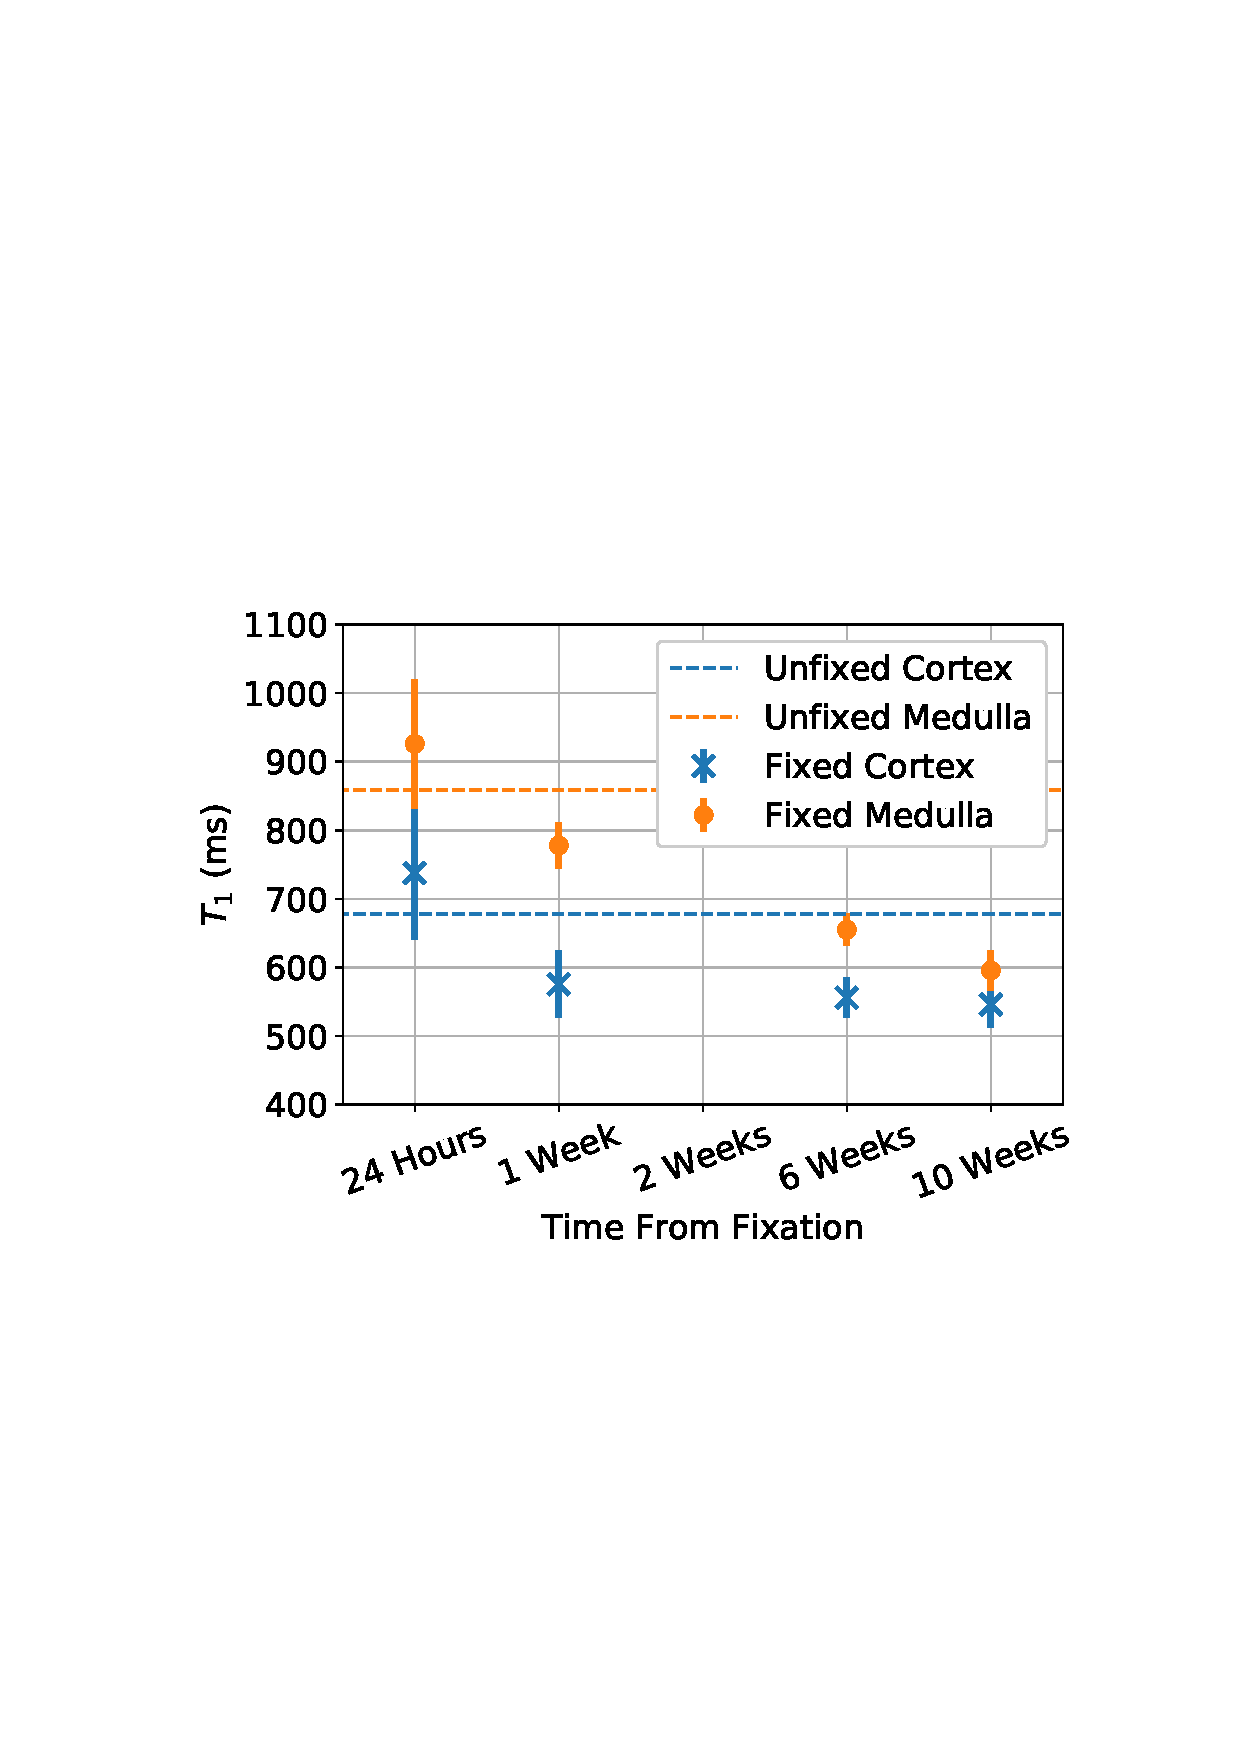
\includegraphics[width=0.47\textwidth]{Neph/T1_3T_crop.pdf}
			\hfill
			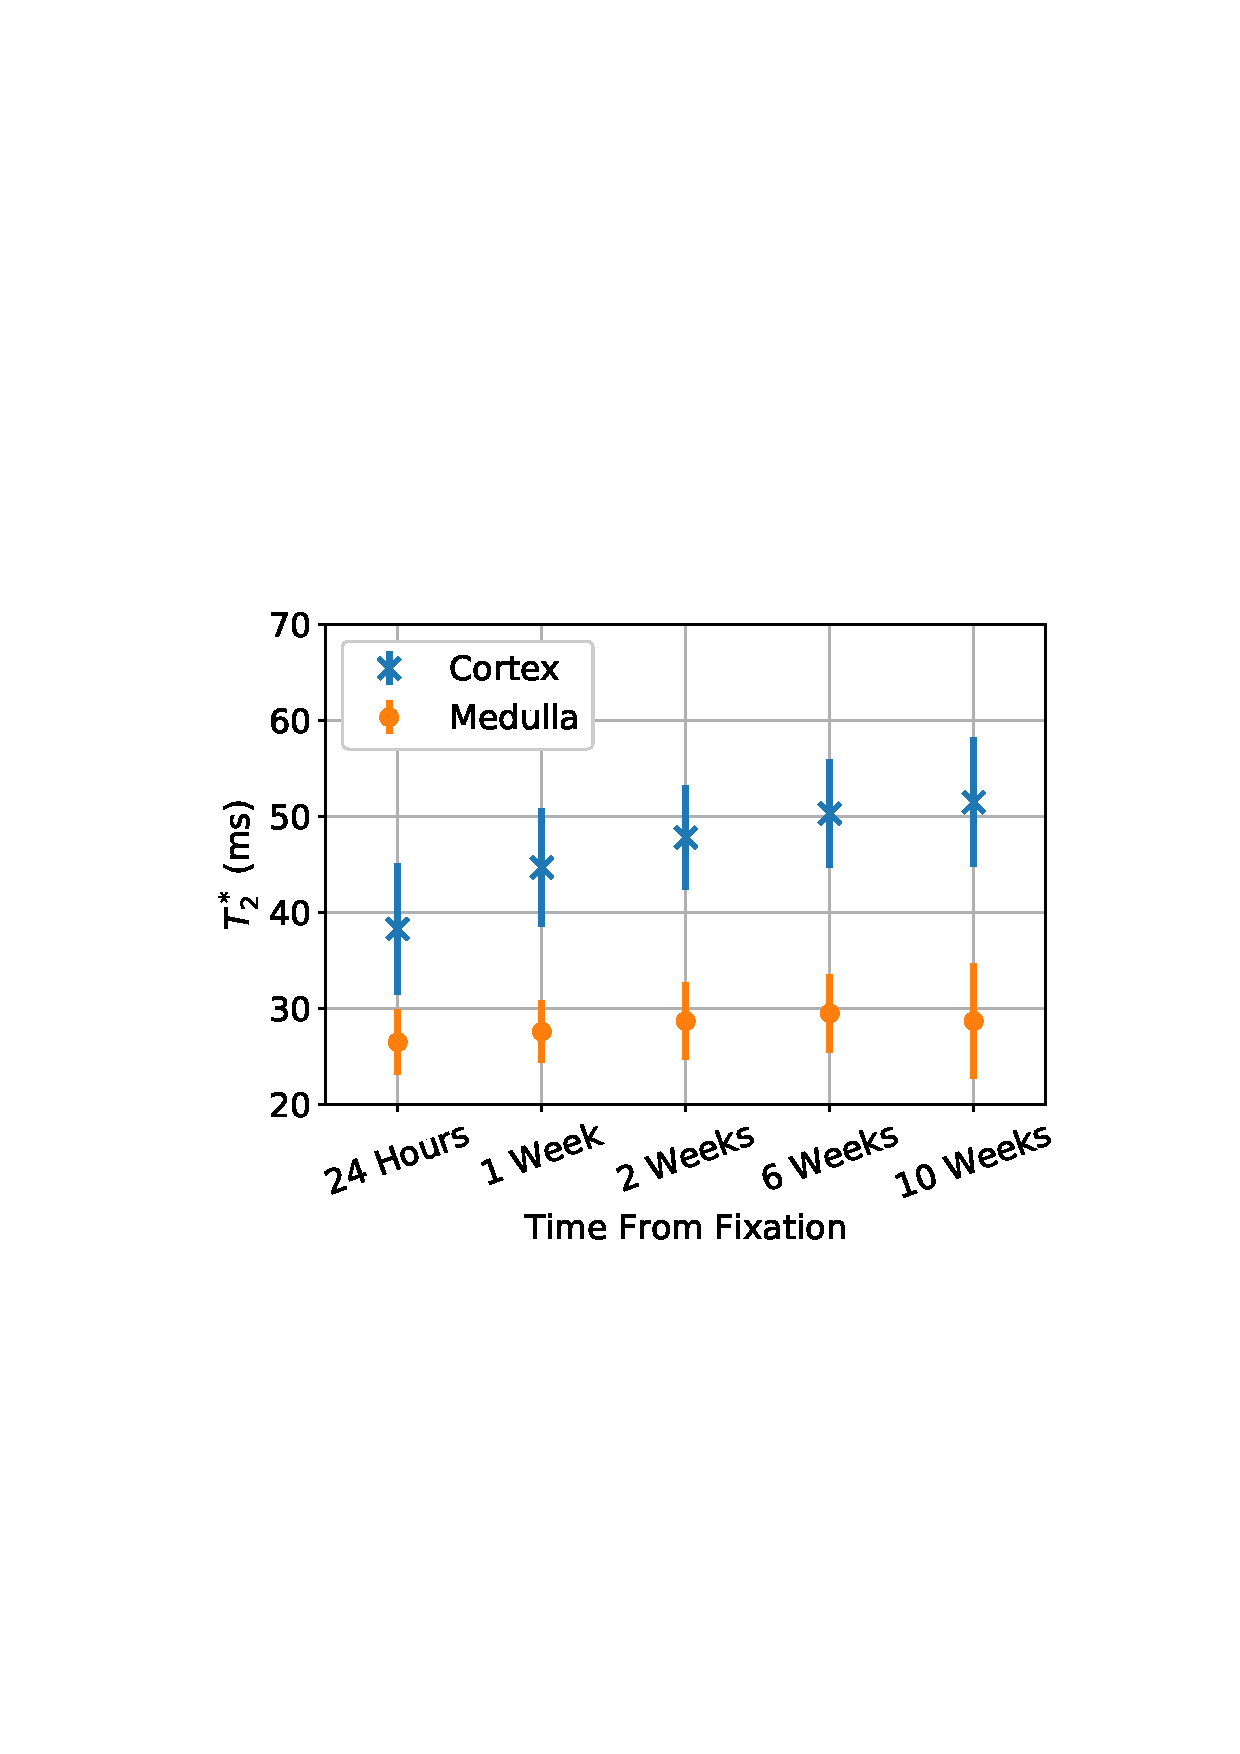
\includegraphics[width=0.47\textwidth]{Neph/T2star_3T_crop.pdf}
			\caption{3T}
			\label{fig:ex_fixation_3t_lts}
		\end{subfigure}
	\end{subfigure}
	\vskip\baselineskip
	\begin{subfigure}[c]{0.9\textwidth}
		\centering
		\begin{subfigure}[c]{1\textwidth}
			\centering
			\includegraphics[width=0.47\textwidth]{Neph/T1_7T_crop.pdf}
			\hfill
			\includegraphics[width=0.47\textwidth]{Neph/T2star_7T_crop.pdf}
			\caption{7T}
			\label{fig:ex_fixation_7t_lts}
		\end{subfigure}
	\end{subfigure}
	\caption{Variation in \tone and \ttwostar at 3T (\subref{fig:ex_fixation_3t_lts}) and 7T (\subref{fig:ex_fixation_7t_lts}). Unfortunately due to technical scanner issues, it was not possible to scan the sample at 7T ten weeks post fixation and the quality of the 3T \tone acquisition two weeks post fixation was significantly inferior; as such these data points have been omitted.}
	\label{fig:ex_fixation_lts}
\end{figure}

Figure \ref{fig:ex_fixation_lts} shows the largest changes in quantitative parameters occurred between twenty four hours and one week after fixation. After this the general trend is that the \tone of the cortex and medulla converge. The \ttwostar of the medulla remains relatively constant while the \ttwostar of the cortex increases and begins to plateau by 10 weeks. In the first week, when the samples have a \tone most similar to that of an unfixed kidney, the quantitative parameters measured will have a dependence on time and as such this necessitates a standardisation in the protocol, specifically the time at which the samples are scanned.

Since it is possible to scan most human samples within twenty four hours of fixation, it was desirable to ascertain how much \tone, \ttwostar and histology change over this period. For this, scanning was only performed at 3T as more frequent measurements were preferable to measurements at different field strengths. For this reason, the number of inversion/echo times collected was reduced to five/six inversion/echo times respectively to fit the protocol into one hour. The choice of \ac{TI} and \ac{TE} was arrived at empirically by calculating maps with every combination of five/six previously acquired \ac{TI}/\ac{TE} and comparing the resultant maps with those calculated using the full complement of inversion and echo times. The reduced protocol consisted of acquisitions with \tone mapping using \acp{TI} of 400 ms, 500 ms, 750 ms, 900 ms, 1100 ms and 2600 ms and \ttwostar mapping using \acp{TE} of 15 ms, 20 ms, 25 ms, 40 ms and 50 ms. The reduction in time points sampled resulted in a mean increase in \tone of $21~\pm~12$~ms and \ttwostar of $0.3 \pm 1.2$~ms compared to the fully sampled protocol.

Scanning sessions commenced at 1.5 hours, 2.5 hours, 4 hours, 5.5 hours, 19 hours and 22 hours after the sample was removed from the \ac{NBF}. Due to the potential for relatively rapid changes in properties, especially \tone, the order in which \ac{TI}/\ac{TE} were collected was randomised rather than ascending/descending order (however this order was kept consistent between scanning sessions). Thus any changes in \tone/\ttwostar over the 30/20 minute acquisition period will manifest themselves as non-systematic noise and thus will simply increase the uncertainty in the fit rather than affecting the calculated value.

To correlate changes with histology at the same time period, the other kidney removed from the animal was biopsied at the start of each of the six scanning session. Mason's trichrome and \ac{H and E} staining was performed on these samples.

Variation in \tone and \ttwostar over the 24 hour period is shown in Figure \ref{fig:ex_fixation_sts}. No significant change in either \tone and \ttwostar was observed, the corresponding histology showed no change in the cortex however there was a noticeable inflammatory response in the medulla. This suggests that the ex-vivo protocol can be performed at any time in the first twenty four hours after fixation and as such makes future experimental logistics simpler.

\begin{figure}[H]
	\centering
	\begin{subfigure}[c]{0.47\textwidth}
		\centering
		%		\missingfigure{T1 vs Times (STS)}
		\includegraphics[width=1\textwidth]{Neph/STS_T1_line.pdf}
		\caption{}
		\label{fig:ex_fixation_t1_3t_sts}
	\end{subfigure}
	\hfill
	\begin{subfigure}[c]{0.47\textwidth}
		\centering
		%		\missingfigure{T2* vs Times (STS)}
		\includegraphics[width=1\textwidth]{Neph/STS_T2star_line.pdf}
		\caption{}
		\label{fig:ex_fixation_t2star_3t_sts}
	\end{subfigure}
	\caption{Changes in \tone (\subref{fig:ex_fixation_t1_3t_sts}) and \ttwostar (\subref{fig:ex_fixation_t2star_3t_sts}) in the first twenty four hours a sample is stored in \ac{PBS} after being fixed in \ac{NBF}.}
	\label{fig:ex_fixation_sts}
\end{figure}

\section{Correlating MRI Measures with Histology in Porcine Kidneys of Differing Ages}
\label{sec:ex_ages}
Kidneys were collected from a 0.5 year old and 2.5 year old pig. These different ages were chosen to assess whether differing levels of renal inflammation and fibrosis is detected. \tone and \ttwostar maps were acquired from both samples and cortical biopsies were removed from the same animals for histological analysis. 

Figure \ref{fig:ex_aged_map} shows example \ac{MRI} data collected from these samples and Figure \ref{fig:ex_aged_bar} shows the quantitative differences in \tone and \ttwo between the kidneys. 

\begin{figure}[H]
	\centering
	\begin{subfigure}[c]{0.47\textwidth}
		\centering
		\includegraphics[width=1\textwidth]{Neph/aged_kidneys/Young_T1.eps}
		\caption{}
		\label{fig:ex_aged_t1_map}
	\end{subfigure}
	\hfill
	\begin{subfigure}[c]{0.47\textwidth}
		\centering
		\includegraphics[width=1\textwidth]{Neph/aged_kidneys/Old_T1.eps}
		\caption{}
		\label{fig:ex_aged_t2star_map}
	\end{subfigure}
	\caption{(\subref{fig:ex_aged_t1_map}) $T_1$ map of a 0.5 year old pig kidney. (\subref{fig:ex_aged_t2star_map}) $T_1$ map of a 2.5 year old pig kidney.}
	\label{fig:ex_aged_map}
\end{figure}

\begin{figure}[H]
	\centering
	\begin{subfigure}[c]{0.47\textwidth}
		\centering
		\includegraphics[width=1\textwidth]{Neph/aged_kidneys/T1_bar.eps}
		\caption{}
		\label{fig:ex_aged_t1_bar}
	\end{subfigure}
	\hfill
	\begin{subfigure}[c]{0.47\textwidth}
		\centering
		\includegraphics[width=1\textwidth]{Neph/aged_kidneys/T2star_bar.eps}
		\caption{}
		\label{fig:ex_aged_t2star_bar}
	\end{subfigure}
	\caption{(\subref{fig:ex_aged_t1_bar}) The $T_1$ of the renal cortex and medulla of the two samples. (\subref{fig:ex_aged_t2star_bar}) The $T_2^*$ of the renal cortex and medulla of the two samples.}
	\label{fig:ex_aged_bar}
\end{figure}

No significant change is observed in the \tone or \ttwostar of the cortex; the medulla of the older kidney had lower \tone. No significant differences were observed in the biopsy samples taken from the renal cortex between the 0.5 year old and 2.5 year old samples, Figure \ref{fig:ex_aged_histo}. This suggests agreement between the \ac{MRI} and histology measurements as neither showed any change in the cortex. 

\begin{figure}[H]
	\centering
	\begin{subfigure}[c]{1\textwidth}
		\centering
		\includegraphics[width=0.8\textwidth]{Neph/aged_kidneys/aged_histo_h_and_e.jpg}
		\caption{}
		\label{fig:ex_aged_histo_h_and_e}
	\end{subfigure}
	\vskip\baselineskip
	\begin{subfigure}[c]{1\textwidth}
		\centering
		\includegraphics[width=0.8\textwidth]{Neph/aged_kidneys/aged_histo_trichrome.jpg}
		\caption{}
		\label{fig:ex_aged_histo_trichrome}
	\end{subfigure}
	\caption{A sample of renal cortex of a 0.5 and 2.5 year old pig stained with (\subref{fig:ex_aged_histo_h_and_e}) \ac{H and E} and (\subref{fig:ex_aged_histo_trichrome}) Masson's trichrome.}
	\label{fig:ex_aged_histo}
\end{figure}

To further investigate how \tone changes with age, kidneys of 1 day old and 4 week old pigs were scanned and compared to histology. Due to their much smaller size, manually segmenting the cortex and medulla of these samples was not possible, as such the depth based analysis outlined in Section \ref{sec:ex_layers} was employed with a layer thickness of 0.5 mm. 

Initially an assessment of consistency between kidneys of the same age was performed. \tone maps of three kidneys from two different animals were generated i.e. both kidneys of one animal and the right kidney of another animal were scanned. In Figure \ref{fig:ex_neo_layers_one_day} excellent agreement between all three kidneys can be seen, with an especially high correlation between kidneys from the same animal. This both gives confidence in the depth based analysis when applied to very small kidneys and indicates that there is a low degree of variance in kidneys of this age.

\begin{figure}[H]
	\centering
	\includegraphics[width=0.8\textwidth]{Neph/aged_kidneys/Neonatal_one_day.pdf}
	\caption{Changes in \tone with renal tissue depth in kidneys of one day old pigs. The shaded area is the standard deviation within each 0.5 mm thick layer of tissue.}
	\label{fig:ex_neo_layers_one_day}	
\end{figure}

The same depth based analysis was applied to a 4 week old kidney and the 0.5 year and 2.5 year old kidneys analysed above. The changes in \tone with depth are shown in Figure \ref{fig:ex_neo_layers_all_ages} both as absolute tissue depth in mm and relative tissue depth in percent, therefore normalising for kidney size. In this figure it can be observed that the \tone of renal tissues differentiates with age. This is in part likely due to decreasing water content with age ($\sim$85~\% in neonatal kidneys, decreasing to $\sim$65-70~\% by adulthood) and in part due to the lower glomerular density in younger kidneys.

\begin{figure}[H]
	\centering
	\begin{subfigure}[c]{0.47\textwidth}
		\centering
		\includegraphics[width=1\textwidth]{Neph/aged_kidneys/Neonatal_all_ages.pdf}
		\caption{}
		\label{fig:ex_neo_layers_all_ages_abs}
	\end{subfigure}
	\hfill
	\begin{subfigure}[c]{0.47\textwidth}
		\centering
		\includegraphics[width=1\textwidth]{Neph/aged_kidneys/Neonatal_all_ages_percent.pdf}
		\caption{}
		\label{fig:ex_neo_layers_all_ages_per}
	\end{subfigure}
	\caption{Changes in \tone with renal depth of pig kidneys of multiple ages. The shaded area is the standard deviation within each 0.5 mm thick layer of tissue. (\subref{fig:ex_neo_layers_all_ages_abs}) shows the absolute depth, (\subref{fig:ex_neo_layers_all_ages_per}) shows the relative depth with 0~\% being the surface of the kidney and 100~\% being the deepest tissue.}
	\label{fig:ex_neo_layers_all_ages}
\end{figure}

% water content
% 1 day old comma and s-shaped bodies
% lower glom density
In future, it would be advantageous to scan samples from older pigs as these will have a greater degree of fibrosis. However, it is not common for pigs to be kept to older ages and so this limits the possibility of highly fibrotic porcine kidneys. Biopsy samples should also include medullary tissue for histological analysis as both Figure \ref{fig:ex_fixation_lts} and Figure \ref{fig:ex_aged_bar} indicate that medullary tissue is relatively variable in quantitative \ac{MRI} and as such, being able to correlate this with histology would be insightful.

\section{Conclusion and Future Work}
Here an ex-vivo protocol has been developed to link with paired and in-vivo quantitative renal \ac{MRI}. This has been developed to provide a pipeline for the assessment of \tone, \ttwo, \ttwostar, \ac{ADC} and \ac{FA} and tractography in the same organ both inside and outside the body. The protocol has validated the effect of fixation time and its use in nephrectomy applications. This protocol can be combined with histological analysis of the samples to link cutting edge \ac{MRI} measures with existing standards for assessment of renal health. Understanding this link will enable \ac{MRI} to augment the current practice of renal biopsys. The highly localised sampling of a biopsy followed by histology can be combined with \acp{MRI} of whole organ coverage to give a better indication of the heterogeneity of renal health.

Further developments were planned in this area but unfortunately the \textsc{covid}-19 pandemic of 2020 limited the availability of samples, access to scanners and a human study of nephrectomy samples with coupled in-vivo and ex-vivo measurements. Firstly, the complete protocol has not been run on a single sample to collect and overlay all quantitative parameters. The correlation of histology and \ac{MRI} data could also be improved. Currently, the histology and imaging data are not registered and as such voxel-by-voxel correlations with histology are not possible. Recently developed software packages focusing on the registration of histology and \ac{MRI} data should assist with this aim \cite{huszar_tensor_2019}. Another area of further development is the ex-vivo \ac{DTI} protocol. There are promising early results, however ex-vivo diffusion imaging poses additional difficulties. During the fixation process, methyl bridges cross link with proteins within the tissue stiffening it and causing a small amount of shrinkage \cite{thavarajah_chemical_2012}. This combined with the lower temperatures of ex-vivo samples ($\sim$ 20$\degree$C room temperature rather than $\sim$ 37$\degree$C body temperature) leads to a reduced degree of diffusion, seen in Figure \ref{fig:ex_adc_maps}. While this results in a higher \ac{SNR} of diffusion sensitised volumes for a given b-value, the underlying diffusion signal being measured is much lower i.e. there is less of a difference between b = 0 s/mm$^2$ and b = 600 sec/mm$^2$ and thus the accuracy of the quantitative maps, Figure \ref{fig:ex_ex_dti_maps}, and tractography, Figure \ref{fig:ex_ex_tracts}, is reduced.

\begin{figure}[H]
	\centering
	\begin{subfigure}[c]{0.31\textwidth}
		\centering
		\includegraphics[width=1\textwidth]{Neph/ex_vivo_fa.png} % 20190923
		\caption{}
		\label{fig:ex_ex_dti_fa}
	\end{subfigure}
	\hfill
	\begin{subfigure}[c]{0.31\textwidth}
		\centering
		\includegraphics[width=1\textwidth]{Neph/ex_vivo_fa_rgb.png} % 20190923
		\caption{}
		\label{fig:ex_ex_dti_fa_rgb}
	\end{subfigure}
	\hfill	
	\begin{subfigure}[c]{0.31\textwidth}
		\centering
		\includegraphics[width=1\textwidth]{Neph/ex_vivo_md.png} % 20190923
		\caption{}
		\label{fig:ex_ex_dti_md}
	\end{subfigure}
	\caption{\ac{FA} (\subref{fig:ex_ex_dti_fa}), fibre direction (\subref{fig:ex_ex_dti_fa_rgb}) and \ac{MD} (\subref{fig:ex_ex_dti_md}) maps of an ex-vivo sample.}
	\label{fig:ex_ex_dti_maps}
\end{figure}

\begin{figure}[H]
	\centering
	\includegraphics[width=0.6\textwidth, angle=270]{Neph/ex_vivo_tracts.png} % 20190923
	\caption{Tractography of an ex-vivo kidney sample.}
	\label{fig:ex_ex_tracts}	
\end{figure}

The ex-vivo protocol presented here could also be used in future to assist stratification of donated organs prior to transplant by scanning organs on cold storage. Organ availability is the limiting factor in renal transplant rate, by increasing confidence in marginal quality organs the time a patient spends on the transplant waiting list could be reduced, reducing risks of complications for the patient due to extended time on dialysis and reduce cost to the health service. This would first require the validation of the effect of temperature on relaxometry measures and the linked histology on discarded organs prior to implementation. The in-vivo protocol could be used to proactively identify dysfunctional grafts and thus modify the course of treatment to extend the life of the transplant.

Future developments will also explore the use of \ac{ASL} on reperfused ex-vivo organs. Reperfusion of the kidney while waiting for a recipient to be matched is an area of intense research \cite{bellini_cold_2019,moers_value_2010,wight_pulsatile_2003}. \ac{ASL} could be used to assess the success of these mechanical perfusion mechanisms and direct improvements in the procedure. Finally \ac{MRI} techniques such as high resolution \ttwostar weighted imaging for the an assessment of glomerular number and density would be an ideal comparison to certain histopathological metrics. While it is not possible to resolve individual glomeruli with the current protocol, other groups in Australia have recently had success applying deep learning and super resolution techniques to enable counting of the glomeruli in a sample at 3T from high resolution \ttwostar weighted data.



\section{Acknowledgements}

I am grateful for access to the University of Nottingham's Augusta high performance computing service. I would also like to thank Prof David Gardner of University of Nottingham Veterinary Science for his assistance with sample acquisition, histopathological processing of samples and general renal physiology expertise. Finally I wish to thank Dr Kevin Aquino for his work in developing 3D depth maps for layer analysis in the brain.

\newpage
\section{References}
\defbibheading{bibliography}[\refname]{}
\printbibliography